\chapter{Perspectives}

My research outlook over the coming decade is going to shift away from studying the Earth's deep interior and move towards the surface. In the next century run-off, which drives fluvial erosion, will likely change significantly due to the effects of global warming on the Earth system. To quote the IPCC's Fifth Assessment Report \cite{IPCC-policy-2014}:

\begin{displayquote}
In many regions, changing precipitation or melting snow and ice are altering hydrological systems, affecting water resources in terms of quantity and quality (medium confidence). Glaciers continue to shrink almost worldwide due to climate change (high confidence), affecting run-off and water resources downstream (medium confidence). Climate change is causing permafrost warming and thawing in high-latitude regions and in high-elevation regions (high confidence).
\end{displayquote}

The impact of such change on sediment storage and transport is uncertain. We can look to the past for evidence of how fluvial systems have responded, but at a time scale of hundreds of years it can become difficult to distinguish the importance of events such as individual storms. Furthermore, as I will expand upon below, there is a broad range of different numerical models developed to study landscape change on different time and spatial scales. One key process is being overlooked: groundwater. Beyond simple empirical laws for 1D infiltration, no numerical models to my knowledge include the impact of groundwater flow on the evolution of fluvial erosion and deposition. Yet rivers recharge by not only by surface run-off but from the ground \citep[e.g.][]{condon-etal-2020}, and river networks most likely grow as a network within the partially saturated ground \citep[e.g.][]{fan-etal-2019}. The challenge is to translate this concept into a testable model that can be applied to fluvial systems.

\section{Short-Term: Non-steady surface water flow}

Landscape evolution modelling on geological time-scales ($>10^{4}$\,yr) has been dominated by one single equation: the stream power law \citep[see][]{howard-1983,howard-1994}. If I return to the simple diagram of surface processes (Figure \ref{fg:1dmodel}), the stream power law makes one very sweeping assumption: the rate of change in sediment thickness within the landscape is zero, which is to say all sediment created is transported out of the model domain. Furthermore, assuming surface flow is the primary driver of landscape erosion and that positive $x$ is in the downstream direction then erosion, $E$, as a function of the power of the flow to detach particles of rock per unit width can be written as,
\begin{equation}
E = -k_{b}\rho_{w}g\mathbf{q}_{w}^{m} \cdot \left(\nabla z\right)^{n},
\label{eq:streampower-inv}
\end{equation}
where $k_{b}$ is a dimensional constant that parametrises bedrock erodability \citep{howard-1983}, $\rho_{w}$ is water density, $g$ is gravity, $q_{w}$ is water flux per unit width, $m$ and $n$ are constants. The exponent $m \sim 0.5$, as it is a function of how the stream flow width is proportional to the water flux \citep[e.g.][]{lacey-1930}. The exponent $n>0$ acts upon the slope. In two dimensions the change in elevation is then given by,
\begin{equation}
\frac{\partial z}{\partial t} = U + k\mathbf{q}_{w}^{m} \cdot \left(\nabla z\right)^{n},
\label{eq:streampower}
\end{equation}
where the constant $k$ lumps together the other constants, and if $n\neq1$ equation \ref{eq:streampower} becomes non-linear. But in any landscape, the assumption of instantaneous sediment transport does not hold. The above model does not work. This raises a question: {\bf what are the key processes within landscape evolution?}

The question of what processes dominates in landscape evolution becomes more important as the time scale of interested becomes shorter. This has lead tot he development of process based landscape evolution models (LEMs) for various applications \citep[see for example][]{temme-etal-2017}. I will briefly describe two that have been used to study landscape change over different time-scales:
\begin{itemize}
\item[1] {\bf LAPSUS}
This is a process based model, where sediment is eroded or deposited down slope based on the transport capacity of the fluvial system \citep{schoorl-etal-2000}. It also includes processes such as soil formation and solid creep. It is a highly simplistic model with eight free parameters which can vary in space and time.
\item[2] {\bf CAESAR-Lisflood}
This is a process based model but of increased complexity compared to LAPSUS. It is based on a cellular automaton approach, but the laws acting on each cell are many and complex. Overland flow is modelled using the Lisflood model of \cite{bates-etal-2010}, and a simple infiltration is included using TOPMODEL \citep{beven-1979}. Subsequently sediment is transported down slope given the shear velocity of the flow is sufficiently high \citep{coulthard-etal-2013,vandeweil-etal-2007}. Other processes are included such as soil creation, lateral erosion, vegetation cover, etc., giving a total of 49 free parameters \citep{skinner-etal-2018}.
\end{itemize}
Given the number of processes typically modelled in LEMs it is difficult to assess which are significant and those to which there is no sensitivity. Recently sensitivity analysis has been carried for CAESAR-Lisflood out using a part of the full parameter space \citep{skinner-etal-2018}. The result of this sensitivity analysis is that the greatest sensitivity was to the sediment transport law, which is a function of the flow of water. This is a first order variable within the model, and it suggests second order aspects such as the degree of vegetation, soil creation are of lower importance.

\begin{figure}
\begin{minipage}{\textwidth}
\begin{minipage}{.5\textwidth}
\includegraphics[width=.98\textwidth]{./figures/ch3-bergantes-elevation.png}
\end{minipage}
\begin{minipage}{.5\textwidth}
\includegraphics[width=.98\textwidth]{./figures/ch3-bergantes-flow.png}
\end{minipage}
\end{minipage}
\caption{Example model evolution of the Riu Bergantes and surrounding area in the Iberian Massif, Spain. The model fLEM is run on the SRTM (Shuttle Radar Topography Mission) DEM (digital elevation model) that includes the Riu Bergantes in the bottom corner ($40^{\circ}$N,$1^{\circ}$W to $41^{\circ}$N,$0^{\circ}$E). The model is run as described in \cite{armitage-2019} for 20\,kyrs, for which the flow field is displayed on the right. No colour bars are shown, as this model is simply a demonstration of the idea rather than a full simulation.}
\label{fg:bergantes}
\end{figure}

To better understand the key processes I am involved in a large project where we plan to compare multiple LEMs on one single catchment, the Riu Bergantes in Spain (Figure \ref{fg:bergantes}). The aim is to take a series of different LEMs: fLEM \citep{armitage-2019}, TISC \citep{garcia-castellanos-2002}, LAPSUS \citep{schoorl-etal-2000}, and CAESAR-Lisflood \citep{coulthard-etal-2013}, and apply them to the same region and explore how they differ in terms of predicted topography and sediment flux. On a smaller scale, in collaboration with Sébastien Rohais, I am currently exploring how the model fLEM and CAESAR-Lisflood compare for modelling sediment transport within the Southern Gulf of Corinth. Key questions are:
\begin{itemize}
    \item[1] What is the impact of large events vs. long-term low magnitude precipitation? It is often assumed that single large events such as floods lead to significant deposition within the sedimentary record. During the last century for example marine cables have suffered significant damage related to turbidite flows. Are these connected with onshore change in precipitation. The two models can be used to explore how precipitation is recorded at the catchment outlet. The advanteage of fLEM is that calculations are rapid, however the water flux term implicitly assumes a steady state flow. CAESAR-Lisflood uses the Lisflood implementation of non-steady water flux, however run times are long. The two models will be used to explore the immpact of the steady / non-steady water flow.
    \item[2] How sensitive are models to the assumed thickness of transportable regolith? In fLEM it is implicitly assumed that there is an infinate supply of material for transport. However, within CAESAR-Lisflood the depth to bedrock can be defined. How will this control the landscape response?
\end{itemize}
  

\section{Long-Term: Groundwater}

\begin{figure}
    \centering
    \includegraphics[width=\textwidth]{./figures/groundwater.png}
    \caption{Left: Diagram showing the major interactions between surface run-off and ground-
water. Precipitation is either routed down slope as surface water, or infiltrates into the
critical zone and deeper groundwater reservoirs. Here it can return to the surface as seepage
into the river network. Middle: The hypothetical conversion of physical properties into seismic paramters. Right: Figure from \cite{clements-2018}: Relating seismic wave speed temporal perturbation to ground water levels. Observed $dv/v$ stacked over all station pairs (black) with modeled $dv/v$ due to thermoelastic strain (dashed) removed compared with groundwater change (blue) in the Baldwin Park Key Well. Grey bars indicate lowest historical water levels of the Baldwin Park Key Well. Blue patches indicate times of drought.}
    \label{fg:groundwater}
\end{figure}

The flow of water is the primary mechanism that transports sediment, weathers rocks and leads to landscape change. Water flows across the surface of the ground in streams and rivers, yet this is only a small proportion of the flow of water. The majority of precipitation infiltrates into the subsurface and flows through the ground from mountain catchments to the river. There are two water worlds, surface water and groundwater (Figure \ref{fg:groundwater}). It is often assumed that erosion is driven by the flow of surface water, and groundwater is ignored within numerical models of landscape evolution (landscape evolution models or LEMs). However recent monitoring of groundwater flow in catchments within for example the Himalayas and Taiwan shows that in fact the main rivers are supplied by groundwater, and this system responds on a timescale that is decoupled from the storm driven rainfall input.

I aim to close these two worlds, and develop the methods to include groundwater flow within LEMs. This is not trivial because the flow of water through variably saturated ground involves solving the non-linear Richards' equation. The challenge is to find the acceptable simplifications that create a solvable system of equations and capture the observed response of groundwater to change in precipitation. This challenge can be met due to recent observations of groundwater with ambient seismic noise. The cross-correlation of seismic noise gives a measure of the change in saturation of the subsurface through time. In the Himalayas this has been used to create a three year continuous history of groundwater flow related to two monsoon cycles. Therefore in this project we will develop a reduced complexity model of groundwater flow that is validated against state-of-the-art observations.

As climate changes it is possible that mountainous catchments will receive increased precipitation and that glaciers will melt at an increasing rate. This surface water will enter the subsurface and impact erosion within the valleys. The impact of this water on aquifer recharge and landscape use is difficult to predict in part because there does not yet exist the tools to model their impact. This project would be a first step to field verified modelling of groundwater coupled to a landscape evolution model. The objectives are:
\begin{itemize}
    \item[1] Develop a reduced complexity model of groundwater flow through the saturated and non-saturated subsurface.
    \item[2] Verify the model against seismic observations of groundwater flow.
\end{itemize}

\subsection{Groundwater and surface water}

The majority of precipitation that falls on the Earth’s surface infiltrates into the vadose zone, the region of the subsurface between the surface and the saturated groundwater reservoir. It then either flows laterally within the upper region of this zone as run-off, is taken up within the soil by organic matter and evaporates (evapotranspiration), or enters the groundwater system. Groundwater then enters the river as a baseflow. The baseflow has, for example, been observed to make up to 37\,\% of the water entering the Liwu River in Taiwan \citep{calmels-etal-2011}. This groundwater is separated between a deep reservoir and a more shallow pathway where the water flows through the upper subsurface (often called the critical zone). These pathways are measured from the major element composition of water, which shows three distinct sources, fast run-off, slow run-off and deep groundwater.

Fast run-off has been traditionally captured in LEMs using a simplification of the shallow water equations. One very popular implementation of this fast run-off driven LEM is Caesar-Lisflood, which is suitable for modelling systems over timescales of decades to centuries \citep{coulthard-etal-2013}. Field observations would suggest that this sort of model captures only two thirds of the water flow, as baseflow is not captured. Hydrological models such as ParFlow solve Richards' equation for the flow of water through variably saturated ground, and therefore can capture the slow run-off and deep groundwater \citep[e.g.][]{jones-2001,maxwell-etal-2015}. Yet, there have been limited efforts in connecting the impact of run-off and groundwater on landscape evolution (c.f.\ Penn State Integrated Hydrologic Model, PIHM; \citep{zhang-etal-2016}. More importantly, the few hydrological models that include subsurface flow have not been compared against field measures of the response of groundwater to change in precipitation.
In this project we will explore the impact of assumptions on the relationship between permeability, saturation, and connectivity on the groundwater flow. Furthermore, there are two key sinks for groundwater, baseflow and evapotranspiration. These two sinks will affect how the system responds to a change in precipitation and infiltration. The key to understanding the role of the two sinks in the groundwater flow is the comparison of model simulations to observations.

\subsection{Simulations to observations}

Groundwater elevation can be measured directly from boreholes. Repeat measurements through time can give an indication of the response of the groundwater system to change in climatic conditions. Continuous monitoring of groundwater levels is possible from the cross-correlation of ambient seismic noise (Figure \ref{fg:groundwater}; \citealp{lecocq-etal-2017,clements-2018}). The saturation of the subsurface changes the seismic properties of the subsurface such that the temporal difference in seismic noise can be used to track change in groundwater saturation. In steep mountain catchments there is evidence that the majority of water enters the river systems via baseflow \citep{jasechko-etal-2016}. Furthermore, as climate changes and glaciers continue to melt, this melt water may increasingly enter the groundwater system rather than entre the river systems directly as run-off \citep{vincent-etal-2019}. Recent work from the Bothe Koshi catchment in the Himalayas would suggest the groundwater responds to monsoon precipitation in two steps, a rapid loss of groundwater due to baseflow post monsoon and a slow loss of groundwater due to evapotranspiration \citep{illien-etal-2020}.

\begin{figure}
    \centering
    \includegraphics[width=\textwidth]{./figures/groundwater-flowchart.png}
    \caption{Flow diagram for forward modelling the seismic response to groundwater movement. On the left is a simplified step by step flow chart that describes the four main processes, (1) treating the input data, (2) developing the flow model, (3) converting the physical parameters to seismic parameters, (4) wave propagation. On the right are the main model equations that need to be solved for the flow and rock physics. There is once central unknown, the hydraulic head, which then gives the saturation and permeability.}
    \label{fg:groundwater-flowchart}
\end{figure}

Non-invasive measure of groundwater levels can be used to verify models of groundwater transport. Rather than interpret the seismic signal, in this project we will build on methods developed for melt flow within the subsurface \citep{franken-etal-2020,armitage-etal-grl-2019} to explore how a model derived synthetic noise cross-correlation is affected by model assumptions of the effects of surface to subsurface water transport (Fiugre \ref{fg:groundwater-flowchart}). The synthetic model space will be converted from physical properties to seismic P and S-wave velocity as a function of saturation and porosity. Using a Biot-Gassmann theory for the effect of three phases, air, water, and solid grains, the seismic velocities can be estimated from the bulk and shear moduli, and density \citep[e.g.][]{rasolofasaon-2012}. This will allow for the forward conversion of physical properties to seismic properties for the forward propagation of seismic waves through the model domain. The synthetic response of ambient seismic noise cross-correlation can then be compared for different model assumptions.

\subsection{Groundwater observations}

A key aspect of this project is to compare the model synthetics to observations. Variations in the seismic velocity with time, $dV/V$, are derived from an inversion algorithm \citep[e.g.][]{lecocq-etal-2017,clements-2018}. There is a significant layer of preprocessing that is applied to the seismic arrivals prior to the inversion. In oreder to compare synthetic models against observations it is therefore important to use the same processing (as I have done for projects relating to mantle-scale seismic tomography and receiver functions, see for example \citealp{goes-etal-2012,armitage-etal-2015,civiero-etal-2019}). At GFZ in Potsdam, Niels Hovius has lead projects within the Boshi Kosi catchment, Nepal (Himalayas). From three years of continuous monitoring, the groundwater response to two monsoon seasons has been inverted \citep{illien-etal-2020}. Therefore in collaboration with GFZ I propose to explore how the forward model compares to the seismic observations.

